\section{Analysis of Solutions: Linear Systems}
While developing the LU Decomposition we have encountered multiple ways a student could implement this method, that is why some discussion associated with which implementation is better should be address.

The multiple ways refers to the critical calculation of the reduction $ A'[row, col+1:n] \gets A'[row, col+1:n] - multiplier \cdot A'[col, col+1:n] $ , those ways could be enumerated as :

\begin{enumerate}
    \item By Submatrices Syntax
    \begin{lstlisting}[language=Python]
A[col + 1 :, col] = A[col + 1 :, col] / pivot
A[col + 1 :, col + 1 :] = A[col + 1 :, col + 1 :] - (A[col + 1 :, :][:, [col]] @ A[[col], :][:, col + 1 :])
    \end{lstlisting}

    \item By New Axis Syntax
    \begin{lstlisting}[language=Python]
A[col + 1 :, col] = A[col + 1 :, col] / pivot
A[col + 1 :, col + 1 :] = A[col + 1 :, col][:, np.newaxis] @ A[col, col + 1 :][np.newaxis, :]
    \end{lstlisting}

    \item By using the Outer Product
    \begin{lstlisting}[language=Python]
A[col + 1 :, col] = A[col + 1 :, col] / pivot
A[col + 1 :, col + 1 :] = np.outer(A[col + 1 :, col], A[col, col + 1 :])
    \end{lstlisting}

    \item By using a for loop
    \begin{lstlisting}[language=Python]
for row in range(col + 1, n):
    A[row, col] = A[row, col] / A[col, col]  # Calculate the multiplier and store in A for later use
    A[row, col + 1 :] = A[row, col + 1 :] - A[row, col] * A[col, col + 1 :]  # Update the remaining elements in the row using the multiplier
    \end{lstlisting} 
\end{enumerate}

To test these methods we will proceed by creating 100 random matrices for the sizes [500, 1000, 1500, 2000, 2500, 3000, 3500, 4000] and measure the length of time it takes for the algorithm to calculate the LU factorisation for each method. Note that all methods have exactly the same syntax before and after the options we have, therefore, we reduce possible noise.
\subsection{Results}
The results of the mean of those 100 iterations for each size in seconds are the following. 
\begin{table}[H]
    \centering
    \begin{tabular}{|l|l|l|l|l|l|}
    \hline
        \textbf{Matrix Size} & \textbf{Submatrices} & \textbf{New Axis} & \textbf{Outer Product} & \textbf{Loop} & \textbf{scipy} \\ \hline
        500 & 0.41335 & 0.169461 & 0.117083 & 0.465405 & 0.018257 \\ \hline
        1000 & 2.563606 & 1.522018 & 1.110119 & 2.176568 & 0.03057 \\ \hline
        1500 & 8.535015 & 5.212411 & 3.8087 & 5.579113 & 0.069611 \\ \hline
        2000 & 20.30588 & 12.333257 & 9.134406 & 10.942175 & 0.132066 \\ \hline
        2500 & 39.145535 & 23.998247 & 17.653031 & 19.098659 & 0.216267 \\ \hline
        3000 & 68.789119 & 41.919219 & 31.590708 & 29.468995 & 0.42402 \\ \hline
        3500 & 106.423081 & 64.700578 & 47.661064 & 42.445734 & 0.447992 \\ \hline
        4000 & 157.028937 & 96.519873 & 70.584879 & 58.448117 & 0.603978 \\ \hline
    \end{tabular}
    \caption{LU Methods Data in seconds}
\end{table}

on a visual plot:

\begin{figure}[H]
  \centering
    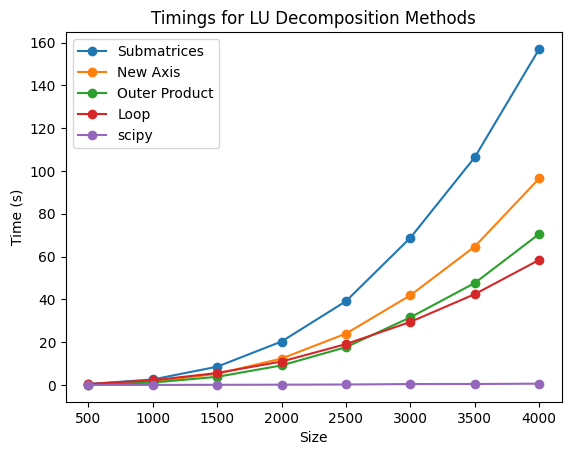
\includegraphics[scale=0.75]{Include/Images/Thesis/Analysis of Solutions/Linear Systems/LU Timings.png}
    \caption{LU Methods comparison}
    \label{fig:LU Methods comparison}
\end{figure}
\begin{figure}[H]
    \centering
    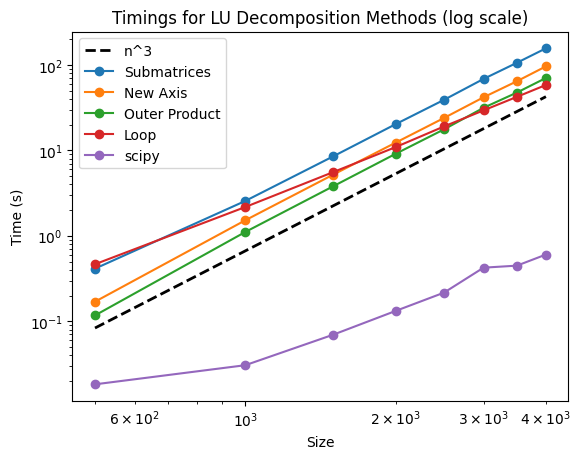
\includegraphics[scale=0.75]{Include/Images/Thesis/Analysis of Solutions/Linear Systems/LU Timings LOG.png}
    \caption{Log plot of LU methods}
    \label{fig:Log plot of LU methods}
\end{figure}

As we can observe from the tabular data and the plot, Scipy's method is by far the fastest, that is, due to the implementation using LAPACK's library, and the slowest is using the Submatrices syntax, surprisingly the syntax using a for-loop improves over the other implementations as size increases, therefore even though this works for large sizes, using a for-loop that implements the reduction is the best choice overall the other methods (without accounting Scipy's) 

For mere due diligence we should also calculate the slope polynomial complexity using simple linear regression
\begin{table}[H]
    \centering
    \begin{tabular}{|l|l|l|l|l|l|}
    \hline
        \textbf{} & \textbf{Submatrices} & \textbf{New Axis} & \textbf{Outer Product} & \textbf{Loop} & \textbf{scipy} \\ \hline
        slope & 2.885234 & 3.043451 & 3.071779 & 2.334054 & 1.813654 \\ \hline
    \end{tabular}
    \caption{LU Data slopes of the polynomial complexity}
\end{table}
In this last table, we can see that although the submatrices syntax was the slowest in the previous plots,is better than using the New Axis syntax, it must be noted that this will be only seen when the size of the matrix is humongous, and barely reachable in a sort span of time. 